% Capitolul 1: Introducere în Analiza Seriilor de Timp
% Prezentare Beamer Cuprinzătoare cu Grafice Generate în Python
% Destinatari: Studenți Master în Statistică și Știința Datelor

\documentclass[9pt, aspectratio=169, t]{beamer}

% Asigură încadrarea conținutului pe diapozitive
\setbeamersize{text margin left=8mm, text margin right=8mm}

%=============================================================================
% CONFIGURARE TEMĂ ȘI STIL
%=============================================================================
\usetheme{Madrid}
\usecolortheme{seahorse}

% Paletă de Culori Inspirată IDA
\definecolor{MainBlue}{RGB}{26, 58, 110}      % IDA Navy Blue
\definecolor{AccentBlue}{RGB}{42, 82, 140}    % Lighter navy
\definecolor{IDAred}{RGB}{220, 53, 69}        % IDA Red
\definecolor{DarkGray}{RGB}{51, 51, 51}
\definecolor{MediumGray}{RGB}{128, 128, 128}
\definecolor{LightGray}{RGB}{248, 248, 248}
\definecolor{VeryLightGray}{RGB}{235, 235, 235}
\definecolor{Crimson}{RGB}{220, 53, 69}
\definecolor{Forest}{RGB}{46, 125, 50}
\definecolor{Amber}{RGB}{181, 133, 63}

\setbeamercolor{palette primary}{bg=MainBlue, fg=white}
\setbeamercolor{palette secondary}{bg=MainBlue!85, fg=white}
\setbeamercolor{palette tertiary}{bg=MainBlue!70, fg=white}
\setbeamercolor{structure}{fg=MainBlue}
\setbeamercolor{title}{fg=MainBlue}
\setbeamercolor{frametitle}{fg=MainBlue, bg=white}
\setbeamercolor{block title}{bg=MainBlue, fg=white}
\setbeamercolor{block body}{bg=VeryLightGray, fg=DarkGray}
\setbeamercolor{block title alerted}{bg=Crimson, fg=white}
\setbeamercolor{block body alerted}{bg=Crimson!8, fg=DarkGray}
\setbeamercolor{block title example}{bg=Forest, fg=white}
\setbeamercolor{block body example}{bg=Forest!8, fg=DarkGray}
\setbeamercolor{item}{fg=MainBlue}

\setbeamertemplate{navigation symbols}{}

\setbeamertemplate{footline}{
    \leavevmode%
    \hbox{%
        \begin{beamercolorbox}[wd=.333333\paperwidth,ht=2.5ex,dp=1ex,center]{author in head/foot}%
            \usebeamerfont{author in head/foot}\insertshortauthor
        \end{beamercolorbox}%
        \begin{beamercolorbox}[wd=.333333\paperwidth,ht=2.5ex,dp=1ex,center]{title in head/foot}%
            \usebeamerfont{title in head/foot}\insertshorttitle
        \end{beamercolorbox}%
        \begin{beamercolorbox}[wd=.333333\paperwidth,ht=2.5ex,dp=1ex,right]{date in head/foot}%
            \usebeamerfont{date in head/foot}\insertshortdate{}\hspace*{2em}
            \insertframenumber{} / \inserttotalframenumber\hspace*{2ex}
        \end{beamercolorbox}}%
    \vskip0pt%
}

%=============================================================================
% PACHETE
%=============================================================================
\usepackage[utf8]{inputenc}
\usepackage[T1]{fontenc}
\usepackage{amsmath, amssymb, amsthm}
\usepackage{mathtools}
\usepackage{bm}
\usepackage{tikz}
\usetikzlibrary{arrows.meta, positioning, shapes, calc}
\usepackage{booktabs}
\usepackage{multirow}
\usepackage{array}
\usepackage{graphicx}
\usepackage{hyperref}
\hypersetup{colorlinks=false, pdfborder={0 0 0}}
\graphicspath{{logos/}{charts/}}

%=============================================================================
% MEDII PENTRU TEOREME
%=============================================================================
\theoremstyle{definition}
\setbeamertemplate{theorems}[numbered]
\newtheorem{defn}{Definiție}
\newtheorem{thm}{Teoremă}
\newtheorem{prop}{Propoziție}
\newtheorem{rmk}{Observație}

%=============================================================================
% COMENZI PERSONALIZATE
%=============================================================================
\newcommand{\E}{\mathbb{E}}
\newcommand{\Var}{\text{Var}}
\newcommand{\Cov}{\text{Cov}}
\newcommand{\Corr}{\text{Corr}}
\newcommand{\R}{\mathbb{R}}
\newcommand{\N}{\mathbb{N}}
\newcommand{\Z}{\mathbb{Z}}

%=============================================================================
% INFORMAȚII TITLU
%=============================================================================
\title[Capitolul 1: Introducere în Serii de Timp]{Capitolul 1: Introducere în Analiza Seriilor de Timp}
\subtitle{Program de licență, Facultatea de Cibernetică, Statistică și Informatică Economică, Academia de Studii Economice din București}
\author[Prof. dr. Daniel Traian Pele]{Prof. dr. Daniel Traian Pele\\[0.2cm]\footnotesize\texttt{danpele@ase.ro}}
\institute{Academia de Studii Economice din București}
\date{An Universitar 2025--2026}

\begin{document}

%=============================================================================
% DIAPOZITIV TITLU
%=============================================================================
\begin{frame}[plain]
    \begin{tikzpicture}[remember picture, overlay]
        \fill[IDAred] (current page.north west) rectangle ([yshift=-0.15cm]current page.north east);
        \node[anchor=north west] at ([xshift=0.5cm, yshift=-0.3cm]current page.north west) {
            \href{https://www.ase.ro}{\includegraphics[height=1.1cm]{ase_logo.png}}
        };
        \node[anchor=north] at ([yshift=-0.3cm]current page.north) {
            \href{https://ai4efin.ase.ro}{\includegraphics[height=1.1cm]{ai4efin_logo.png}}
        };
        \node[anchor=north east] at ([xshift=-0.5cm, yshift=-0.3cm]current page.north east) {
            \href{https://www.digital-finance-msca.com}{\includegraphics[height=1.1cm]{msca_logo.png}}
        };
    \end{tikzpicture}
    \vfill
    \begin{center}
        {\Huge\textbf{\textcolor{MainBlue}{Capitolul 1: Introducere în Serii de Timp}}}\\[0.5cm]
        {\Large\textcolor{IDAred}{Fundamente și Concepte}}
    \end{center}
    \vfill

    \begin{tikzpicture}[remember picture, overlay]
        \fill[IDAred] (current page.south west) rectangle ([yshift=0.15cm]current page.south east);
        \node[anchor=south west] at ([xshift=0.5cm, yshift=0.8cm]current page.south west) {
            \href{https://theida.net}{\includegraphics[height=0.9cm]{ida_logo.png}}
        };
        \node[anchor=south] at ([xshift=-3cm, yshift=0.8cm]current page.south) {
            \href{https://blockchain-research-center.com}{\includegraphics[height=0.9cm]{brc_logo.png}}
        };
        \node[anchor=south] at ([yshift=0.8cm]current page.south) {
            \href{https://quantinar.com}{\includegraphics[height=0.9cm]{qr_logo.png}}
        };
        \node[anchor=south] at ([xshift=3cm, yshift=0.8cm]current page.south) {
            \href{https://quantlet.com}{\includegraphics[height=0.9cm]{ql_logo.png}}
        };
        \node[anchor=south east] at ([xshift=-0.5cm, yshift=0.8cm]current page.south east) {
            \href{https://ipe.ro/new}{\includegraphics[height=0.9cm]{acad_logo.png}}
        };
    \end{tikzpicture}
\end{frame}

%=============================================================================
% OBIECTIVELE CURSULUI
%=============================================================================
\begin{frame}{Obiective de Învățare}
    \textbf{\large La sfârșitul acestui capitol, veți fi capabili să:}
    \vspace{0.15cm}
    \begin{enumerate}
        \item[\textcolor{MainBlue}{\textbf{1.}}] \textbf{Definiți} seriile de timp și să le distingeți de datele transversale și de panel
        \vspace{0.08cm}
        \item[\textcolor{MainBlue}{\textbf{2.}}] \textbf{Descompuneți} seriile de timp în componente de trend, sezonalitate și reziduuri
        \vspace{0.08cm}
        \item[\textcolor{MainBlue}{\textbf{3.}}] \textbf{Aplicați} netezirea exponențială (SES, Holt, Holt-Winters, ETS)
        \vspace{0.08cm}
        \item[\textcolor{MainBlue}{\textbf{4.}}] \textbf{Evaluați} prognozele folosind MAE, RMSE, MAPE; separări train/validare/test
        \vspace{0.08cm}
        \item[\textcolor{MainBlue}{\textbf{5.}}] \textbf{Modelați} sezonalitatea folosind variabile dummy sau termeni Fourier
        \vspace{0.08cm}
        \item[\textcolor{MainBlue}{\textbf{6.}}] \textbf{Gestionați} trendul și sezonalitatea prin detrendare și ajustare
        \vspace{0.08cm}
        \item[\textcolor{MainBlue}{\textbf{7.}}] \textbf{Înțelegeți} procesele stocastice și staționaritatea
        \vspace{0.08cm}
        \item[\textcolor{MainBlue}{\textbf{8.}}] \textbf{Calculați} ACF/PACF și efectuați teste de staționaritate (ADF, KPSS)
    \end{enumerate}
\end{frame}

%=============================================================================
% CUPRINS
%=============================================================================
\begin{frame}{Structura Capitolului}
    \tableofcontents
\end{frame}

%=============================================================================
% MOTIVAȚIE
%=============================================================================
\begin{frame}{Seriile de Timp Sunt Pretutindeni}
    \vspace{-0.3cm}
    \begin{center}
        \includegraphics[width=0.92\textwidth, height=0.62\textheight, keepaspectratio]{charts/ch1_motivation_everywhere.pdf}
    \end{center}
    \vspace{-0.2cm}
    {\footnotesize
    \begin{itemize}
        \item \textbf{Finanțe}: Prețuri de acțiuni, cursuri de schimb, volume de tranzacționare
        \item \textbf{Economie}: PIB, șomaj, rate ale inflației
        \item \textbf{Afaceri}: Vânzări, trafic web, cererea clienților
        \item \textbf{Știință}: Temperatură, niveluri de poluare, indicatori vitali ai pacienților
    \end{itemize}
    }
\end{frame}

\begin{frame}{De Ce Studiem Seriile de Timp?}
    \vspace{-0.3cm}
    \begin{center}
        \includegraphics[width=0.92\textwidth, height=0.62\textheight, keepaspectratio]{charts/ch1_motivation_forecast.pdf}
    \end{center}
    \vspace{-0.2cm}
    {\footnotesize
    \begin{alertblock}{Obiectivul Principal: Prognoza}
        Folosiți tiparele istorice pentru a prezice valorile viitoare --- esențial pentru planificarea afacerilor, gestionarea riscurilor și deciziile de politică.
    \end{alertblock}
    }
\end{frame}

\begin{frame}{Înțelegerea Structurii Seriilor de Timp}
    \vspace{-0.3cm}
    \begin{center}
        \includegraphics[width=0.92\textwidth, height=0.60\textheight, keepaspectratio]{charts/ch1_motivation_components.pdf}
    \end{center}
    \vspace{-0.2cm}
    {\footnotesize
    \begin{exampleblock}{Descompunere}
        Orice serie de timp poate fi descompusă în componente interpretabile: trend, sezonalitate și zgomot.
    \end{exampleblock}
    }
\end{frame}

%=============================================================================
% SECȚIUNEA 1: CE ESTE O SERIE DE TIMP
%=============================================================================
\section{Ce Este o Serie de Timp?}

\begin{frame}{Definiția unei Serii de Timp}
    \begin{defn}[Serie de Timp]
        O \textbf{serie de timp} este o secvență de observații $\{X_t\}$ indexate după timp:
        \[
            \{X_t : t \in \mathcal{T}\}
        \]
        unde $\mathcal{T}$ este un set de indici reprezentând puncte temporale.
    \end{defn}

    \vspace{0.15cm}

    \textbf{Caracteristici cheie:}
    \begin{itemize}
        \item \textbf{Ordonate}: Observațiile au o ordine temporală naturală
        \item \textbf{Dependente}: Observațiile consecutive sunt de obicei corelate
        \item \textbf{Discrete} sau \textbf{Continue}: Indexul temporal poate fi discret ($t = 1, 2, 3, \ldots$) sau continuu
    \end{itemize}

    \vspace{0.15cm}

    \textbf{Notație:}
    \begin{itemize}
        \item $X_t$ = observația la momentul $t$
        \item $\{X_t\}_{t=1}^{T}$ = serie de timp finită cu $T$ observații
    \end{itemize}
\end{frame}

\begin{frame}{Serie de Timp: Ilustrație Vizuală}
    \begin{center}
        \includegraphics[width=0.85\textwidth]{charts/ch1_def_timeseries.pdf}
    \end{center}
    \vspace{0.2cm}
    \small Fiecare punct $X_t$ reprezintă o observație la momentul $t$. Secvența este ordonată și observațiile consecutive sunt de obicei corelate.
\end{frame}

\begin{frame}{Tipare Comune în Seriile de Timp}
    \vspace{-0.3cm}
    \begin{center}
        \includegraphics[width=0.82\textwidth, height=0.58\textheight, keepaspectratio]{charts/ch1_ts_patterns.pdf}
    \end{center}
    \vspace{-0.2cm}
    {\footnotesize
    \begin{itemize}
        \item \textbf{Trend}: Creștere sau scădere pe termen lung a datelor
        \item \textbf{Sezonalitate}: Tipare periodice regulate (de ex., lunar, trimestrial)
        \item \textbf{Aleatoriu}: Niciun tipar sistematic -- fluctuații imprevizibile
    \end{itemize}
    }
\end{frame}

\begin{frame}{Serie de Timp: Definiție Vizuală}
    \begin{center}
        \includegraphics[width=0.78\textwidth]{timeseries_definition.pdf}
    \end{center}
    \vspace{-0.2cm}
    \small Fiecare punct $X_t$ reprezintă o măsurătoare la momentul discret $t$. Date: S\&P 500 (2024).
\end{frame}

\begin{frame}{Tipuri de Date: Comparație}
    \begin{center}
        \includegraphics[width=0.78\textwidth]{data_types_comparison.pdf}
    \end{center}

    \vspace{0.2cm}
    \begin{center}
    \small
    \begin{tabular}{lccc}
        \toprule
        \textbf{Tip de Date} & \textbf{Unități ($N$)} & \textbf{Timp ($T$)} & \textbf{Exemplu} \\
        \midrule
        Transversale & Multe & 1 & Sondaj pe 1000 gospodării \\
        Serie de timp & 1 & Multe & Prețuri zilnice S\&P 500 \\
        Panel & Multe & Multe & PIB pentru 50 țări, 20 ani \\
        \bottomrule
    \end{tabular}
    \end{center}
\end{frame}

\begin{frame}{Exemple de Date de Tip Serie de Timp}
    \begin{center}
        \includegraphics[width=0.78\textwidth]{multiple_assets.pdf}
    \end{center}
    \vspace{-0.2cm}
    \centering\small Date financiare reale de la Yahoo Finance (2019--2025). Normalizate la baza 100.
\end{frame}

%=============================================================================
% SECȚIUNEA 2: DESCOMPUNEREA SERIILOR DE TIMP
%=============================================================================
\section{Descompunerea Seriilor de Timp}

\begin{frame}{De Ce Descompunem o Serie de Timp?}
    \textbf{Descompunerea} separă o serie de timp în componente interpretabile:

    \vspace{0.15cm}

    \begin{columns}[T]
        \begin{column}{0.48\textwidth}
            \textbf{Obiective:}
            \begin{itemize}
                \item Înțelegerea tiparelor subiacente
                \item Eliminarea sezonalității pentru modelare
                \item Identificarea direcției trendului
                \item Izolarea fluctuațiilor neregulate
                \item Îmbunătățirea acurateței prognozei
            \end{itemize}
        \end{column}
        \begin{column}{0.48\textwidth}
            \textbf{Componente:}
            \begin{itemize}
                \item $T_t$ = \textbf{Trend}: Mișcare pe termen lung
                \item $S_t$ = \textbf{Sezonalitate}: Tipar periodic regulat
                \item $C_t$ = \textbf{Ciclic}: Fluctuații ale ciclului de afaceri
                \item $\varepsilon_t$ = \textbf{Rezidual}: Zgomot aleatoriu
            \end{itemize}
        \end{column}
    \end{columns}

    \vspace{0.2cm}

    \begin{block}{Modele Clasice de Descompunere}
        \begin{itemize}
            \item \textbf{Aditiv}: $X_t = T_t + S_t + \varepsilon_t$
            \item \textbf{Multiplicativ}: $X_t = T_t \times S_t \times \varepsilon_t$
        \end{itemize}
    \end{block}
\end{frame}

\begin{frame}{Descompunerea Seriilor de Timp: Exemplu Vizual}
    \vspace{-0.3cm}
    \begin{center}
        \includegraphics[width=0.82\textwidth, height=0.58\textheight, keepaspectratio]{charts/ch1_decomposition.pdf}
    \end{center}
    \vspace{-0.2cm}
    {\footnotesize
    \begin{itemize}
        \item \textbf{Original}: Seria de timp observată cu toate componentele
        \item \textbf{Trend}: Mișcarea subiacentă pe termen lung extrasă prin netezire
        \item \textbf{Sezonalitate}: Tiparul periodic regulat care se repetă la fiecare ciclu
        \item \textbf{Rezidual}: Zgomotul aleatoriu după eliminarea trendului și sezonalității
    \end{itemize}
    }
\end{frame}

\begin{frame}{Componenta Ciclică}
    \textbf{Componenta ciclică} $C_t$: Fluctuații pe termen mediu (2--10 ani)

    \vspace{0.15cm}

    \begin{columns}[T]
        \begin{column}{0.48\textwidth}
            \textbf{Caracteristici:}
            \begin{itemize}
                \item Fluctuații ale ciclului de afaceri
                \item Nicio perioadă fixă (spre deosebire de sezonalitate)
                \item Durata variază: 2--10 ani
                \item Amplitudinea variază în timp
            \end{itemize}
        \end{column}
        \begin{column}{0.48\textwidth}
            \textbf{Exemple:}
            \begin{itemize}
                \item Expansiuni/recesiuni economice
                \item Cicluri de credit
                \item Cicluri imobiliare
                \item Cicluri ale prețurilor materiilor prime
            \end{itemize}
        \end{column}
    \end{columns}

    \vspace{0.15cm}

    \begin{alertblock}{Notă Practică}
        Adesea combinată cu trendul ca componentă \textbf{trend-ciclu} deoarece:
        \begin{itemize}
            \item Dificil de separat de trend cu date scurte
            \item Multe metode de descompunere estimează $T_t + C_t$ împreună
        \end{itemize}
    \end{alertblock}
\end{frame}

\begin{frame}{Modelul de Descompunere Aditivă}
    \textbf{Formula:} \quad $X_t = T_t + S_t + \varepsilon_t$

    \vspace{0.15cm}

    \textbf{Când se utilizează:}
    \begin{itemize}
        \item Fluctuațiile sezoniere sunt \textbf{constante} în timp
        \item Varianța seriei este \textbf{stabilă}
    \end{itemize}

    \vspace{0.15cm}

    \textbf{Proprietăți:}
    \begin{itemize}
        \item $\E[\varepsilon_t] = 0$ (reziduuri cu medie zero)
        \item $\sum_{j=1}^{s} S_j = 0$ (sezonalitatea însumează la zero)
        \item Unitățile lui $S_t$ sunt aceleași cu ale lui $X_t$
    \end{itemize}
\end{frame}

\begin{frame}{Descompunere Aditivă: Vizualizare}
    \begin{center}
        \includegraphics[width=0.78\textwidth]{ts_components_synthetic.pdf}
    \end{center}
\end{frame}

\begin{frame}{Modelul de Descompunere Multiplicativă}
    \textbf{Formula:} \quad $X_t = T_t \times S_t \times \varepsilon_t$

    \vspace{0.15cm}

    \textbf{Când se utilizează:}
    \begin{itemize}
        \item Fluctuațiile sezoniere \textbf{cresc} odată cu nivelul seriei
        \item Varianța \textbf{crește} în timp
    \end{itemize}

    \vspace{0.15cm}

    \textbf{Proprietăți:}
    \begin{itemize}
        \item $\E[\varepsilon_t] = 1$ (reziduuri centrate la 1)
        \item $\frac{1}{s}\sum S_j = 1$ (media sezonalității este 1)
        \item $S_t$ este un raport (adimensional)
    \end{itemize}

    \vspace{0.15cm}

    \textbf{Sfat:} Transformarea logaritmică convertește la modelul aditiv.
\end{frame}

\begin{frame}{Descompunere Multiplicativă: Date Reale}
    \begin{center}
        \includegraphics[width=0.72\textwidth]{airline_decomposition.pdf}
    \end{center}
    \vspace{-0.3cm}
    \centering\small Setul de date clasic Box-Jenkins pentru pasageri aerieni (1949--1960).
\end{frame}

\begin{frame}{Aditivă vs Multiplicativă: Comparație}
    \begin{center}
        \includegraphics[width=0.78\textwidth]{additive_vs_multiplicative.pdf}
    \end{center}

    \vspace{0.2cm}
    \small\textbf{Diferența cheie:} În modelul multiplicativ, componenta sezonală este un \textit{raport} (centrat la 1), în timp ce în modelul aditiv este în \textit{unități absolute} (centrat la 0).
\end{frame}

\begin{frame}{Estimarea Trendului: Media Mobilă}
    \begin{defn}[Media Mobilă Centrată]
        \textbf{Media mobilă centrată} de ordin $2q+1$ este:
        \[
            \hat{T}_t = \frac{1}{2q+1} \sum_{j=-q}^{q} X_{t+j}
        \]
    \end{defn}

    \vspace{0.2cm}

    \textbf{Pentru date sezoniere:}
    \begin{itemize}
        \item Dacă perioada $s$ este \textbf{impară}: medie simplă pe $s$ observații
        \item Dacă perioada $s$ este \textbf{pară} (de ex., 12): se folosește MA $2 \times s$ cu ponderi înjumătățite la capete
    \end{itemize}

    \vspace{0.2cm}

    \textbf{Proprietăți:}
    \begin{itemize}
        \item Netezește fluctuațiile sezoniere și aleatorii
        \item Fereastră mai mare $\Rightarrow$ trend mai neted
        \item Compromis: pierdere de date la capete
    \end{itemize}
\end{frame}

\begin{frame}{Media Mobilă Centrată: Ilustrație Vizuală}
    \begin{center}
        \includegraphics[width=0.9\textwidth]{charts/ch1_def_moving_average.pdf}
    \end{center}
    \vspace{-0.2cm}
    \small Media mobilă netezește fluctuațiile pe termen scurt, dezvăluind trendul subiacent.
\end{frame}

\begin{frame}{Algoritmul Descompunerii Clasice}
    \textbf{Pași pentru Descompunerea Multiplicativă:}

    \vspace{0.2cm}

    \begin{enumerate}
        \item \textbf{Estimarea Trendului}: $\hat{T}_t = MA_s(X_t)$

        \vspace{0.15cm}

        \item \textbf{Detrendare}: $D_t = X_t / \hat{T}_t$

        \vspace{0.15cm}

        \item \textbf{Estimarea Sezonalității}: Media $D_t$ pentru fiecare sezon $j$
        \[
            \hat{S}_j = \text{media}(D_t \text{ pentru toate } t \text{ din sezonul } j)
        \]

        \vspace{0.15cm}

        \item \textbf{Normalizare}: Scalare astfel încât $\frac{1}{s}\sum_{j=1}^{s} \hat{S}_j = 1$

        \vspace{0.15cm}

        \item \textbf{Calculul Reziduurilor}: $\hat{\varepsilon}_t = X_t / (\hat{T}_t \times \hat{S}_t)$
    \end{enumerate}
\end{frame}

\begin{frame}{Indici Sezonieri: Interpretare}
    \begin{center}
        \includegraphics[width=0.78\textwidth]{seasonal_pattern.pdf}
    \end{center}

    \vspace{0.2cm}
    \small\textbf{Interpretare:} $S_t > 1$ înseamnă activitate peste medie; $S_t < 1$ înseamnă sub medie. Datele aeriene arată vârf de călătorii în iulie--august.
\end{frame}

\begin{frame}{Descompunerea STL: O Abordare Modernă}
    \begin{defn}[STL - Descompunere Sezonieră-Trend folosind LOESS]
        \textbf{STL} folosește regresia ponderată local (LOESS) pentru a estima componentele:
        \[
            X_t = T_t + S_t + R_t
        \]
    \end{defn}

    \vspace{0.2cm}

    \textbf{Avantaje față de descompunerea clasică:}
    \begin{itemize}
        \item Gestionează \textbf{orice perioadă sezonieră} (nu doar 4 sau 12)
        \item Componenta sezonieră poate \textbf{să se schimbe în timp}
        \item \textbf{Robust} la valori aberante (cu opțiunea robust=True)
        \item Oferă estimări \textbf{netede} ale trendului
    \end{itemize}

    \vspace{0.2cm}

    \textbf{Parametri cheie:}
    \begin{itemize}
        \item \texttt{period}: Perioada sezonieră (de ex., 12 pentru lunar)
        \item \texttt{seasonal}: Fereastră pentru netezirea sezonieră (întreg impar)
        \item \texttt{robust}: Folosește ajustare robustă pentru a reduce ponderea valorilor aberante
    \end{itemize}
\end{frame}

\begin{frame}{Descompunerea STL: Ilustrație Vizuală}
    \begin{center}
        \includegraphics[width=0.85\textwidth]{charts/ch1_def_stl.pdf}
    \end{center}
    \vspace{-0.2cm}
    \small STL separă seria originală în componente de trend, sezonalitate și rest folosind regresia ponderată local.
\end{frame}

%=============================================================================
% SECȚIUNEA 3: METODE DE NETEZIRE EXPONENȚIALĂ
%=============================================================================
\section{Metode de Netezire Exponențială}

\begin{frame}{Netezirea Exponențială: Prezentare Generală}
    Metodele de \textbf{netezire exponențială} produc prognoze bazate pe medii ponderate ale observațiilor trecute, cu ponderi care scad exponențial.

    \vspace{0.15cm}

    \begin{block}{De Ce Netezire Exponențială?}
        \begin{itemize}
            \item Metode de prognoză simple dar eficiente
            \item Observațiile mai recente primesc ponderi mai mari
            \item Gestionează trendul și sezonalitatea
            \item Baza pentru modelele ETS
        \end{itemize}
    \end{block}

    \vspace{0.15cm}

    \textbf{Trei metode principale:}
    \begin{enumerate}
        \item \textbf{Netezire Exponențială Simplă (SES)}: Doar nivel
        \item \textbf{Metoda Holt}: Nivel + Trend
        \item \textbf{Holt-Winters}: Nivel + Trend + Sezonalitate
    \end{enumerate}
\end{frame}

\begin{frame}{Netezirea cu Media Mobilă}
    \vspace{-0.3cm}
    \begin{center}
        \includegraphics[width=0.82\textwidth, height=0.58\textheight, keepaspectratio]{charts/ch1_moving_average.pdf}
    \end{center}
    \vspace{-0.2cm}
    {\footnotesize
    \begin{itemize}
        \item \textbf{Fereastră mică} (de ex., 5): Receptivă la schimbări dar zgomotoasă
        \item \textbf{Fereastră mare} (de ex., 30): Mai netedă dar mai lentă în reacție
        \item Compromis între reducerea zgomotului și întârzierea în detectarea schimbărilor
    \end{itemize}
    }
\end{frame}

\begin{frame}{Netezirea Exponențială Simplă (SES)}
    \textbf{Prognoză:} \quad $\hat{X}_{t+1|t} = \alpha X_t + (1-\alpha)\hat{X}_{t|t-1}$

    \vspace{0.15cm}

    unde $\alpha \in (0,1)$ este \textbf{parametrul de netezire}.

    \vspace{0.15cm}

    \textbf{Cum funcționează:}
    \begin{itemize}
        \item Ponderile scad exponențial în trecut
        \item $\alpha$ mare: receptiv la schimbările recente
        \item $\alpha$ mic: prognoze mai netede, mai stabile
    \end{itemize}

    \vspace{0.15cm}

    \textbf{Forma de nivel:} \quad $\ell_t = \alpha X_t + (1-\alpha)\ell_{t-1}$
\end{frame}

\begin{frame}{Netezirea Exponențială: Efectul lui Alpha}
    \vspace{-0.3cm}
    \begin{center}
        \includegraphics[width=0.82\textwidth, height=0.58\textheight, keepaspectratio]{charts/ch1_exponential_smoothing.pdf}
    \end{center}
    \vspace{-0.2cm}
    {\footnotesize
    \begin{itemize}
        \item \textbf{$\alpha$ mic} (de ex., 0.1): Mai multă pondere pe trecut -- mai neted, adaptare mai lentă
        \item \textbf{$\alpha$ mare} (de ex., 0.9): Mai multă pondere pe recent -- receptiv, mai volatil
        \item Alegeți $\alpha$ în funcție de cât de rapid se schimbă procesul subiacent
    \end{itemize}
    }
\end{frame}

\begin{frame}{Netezirea Exponențială Simplă: Efectul lui $\alpha$}
    \begin{center}
        \includegraphics[width=0.78\textwidth]{simple_exp_smoothing.pdf}
    \end{center}
    \vspace{-0.2cm}
    \small Un $\alpha$ mai mic produce prognoze mai netede; un $\alpha$ mai mare urmează datele mai îndeaproape.
\end{frame}

\begin{frame}{Metoda Holt cu Trend Liniar}
    Extinde SES pentru a captura \textbf{trendul liniar} folosind două ecuații:

    \vspace{0.15cm}

    \textbf{Nivel:} \quad $\ell_t = \alpha X_t + (1-\alpha)(\ell_{t-1} + b_{t-1})$

    \vspace{0.2cm}

    \textbf{Trend:} \quad $b_t = \beta^*(\ell_t - \ell_{t-1}) + (1-\beta^*)b_{t-1}$

    \vspace{0.15cm}

    \textbf{Prognoză:} \quad $\hat{X}_{t+h|t} = \ell_t + h \cdot b_t$

    \vspace{0.15cm}

    \textbf{Parametri:}
    \begin{itemize}
        \item $\alpha \in (0,1)$: Parametru de netezire pentru nivel
        \item $\beta^* \in (0,1)$: Parametru de netezire pentru trend
        \item $\ell_t$: Nivelul estimat la momentul $t$
        \item $b_t$: Trendul (panta) estimat la momentul $t$
    \end{itemize}
\end{frame}

\begin{frame}{Metoda Holt: Vizualizare}
    \begin{center}
        \includegraphics[width=0.78\textwidth]{holt_method.pdf}
    \end{center}
    \vspace{-0.2cm}
    \small Metoda Holt captează atât nivelul cât și trendul, proiectându-le în orizontul de prognoză.
\end{frame}

\begin{frame}{Metoda Sezonieră Holt-Winters}
    Extinde metoda Holt pentru a include \textbf{sezonalitatea} cu trei ecuații:

    \vspace{0.2cm}

    \textbf{Nivel:} \quad $\ell_t = \alpha(X_t - S_{t-s}) + (1-\alpha)(\ell_{t-1} + b_{t-1})$

    \vspace{0.1cm}

    \textbf{Trend:} \quad $b_t = \beta^*(\ell_t - \ell_{t-1}) + (1-\beta^*)b_{t-1}$

    \vspace{0.1cm}

    \textbf{Sezonalitate:} \quad $S_t = \gamma(X_t - \ell_t) + (1-\gamma)S_{t-s}$

    \vspace{0.15cm}

    \textbf{Prognoză:} \quad $\hat{X}_{t+h|t} = \ell_t + h \cdot b_t + S_{t+h-s(k+1)}$

    \vspace{0.15cm}

    \textbf{Parametri:}
    \begin{itemize}
        \item $\alpha$: Netezire nivel
        \item $\beta^*$: Netezire trend
        \item $\gamma$: Netezire sezonalitate
        \item $s$: Perioada sezonieră (de ex., 12 pentru lunar)
    \end{itemize}
\end{frame}

\begin{frame}{Holt-Winters: Captarea Sezonalității}
    \begin{center}
        \includegraphics[width=0.78\textwidth]{holt_winters.pdf}
    \end{center}
    \vspace{-0.2cm}
    \small Holt-Winters descompune seria și produce prognoze sezoniere.
\end{frame}

\begin{frame}{Cadrul ETS: Eroare-Trend-Sezonalitate}
    \begin{defn}[Modele ETS]
        Cadrul \textbf{ETS} generalizează netezirea exponențială cu structură explicită de eroare:
        \[
            \text{ETS}(E, T, S)
        \]
        unde fiecare componentă poate fi:
    \end{defn}

    \vspace{0.2cm}

    \begin{center}
    \small
    \begin{tabular}{llll}
        \toprule
        \textbf{Componentă} & \textbf{N} & \textbf{A} & \textbf{M} \\
        \midrule
        Eroare (E) & -- & Aditivă & Multiplicativă \\
        Trend (T) & Niciunul & Aditiv & Multiplicativ \\
        Sezonalitate (S) & Niciuna & Aditivă & Multiplicativă \\
        \bottomrule
    \end{tabular}
    \end{center}

    \vspace{0.2cm}

    \textbf{Exemple:}
    \begin{itemize}
        \item ETS(A,N,N) = Netezire Exponențială Simplă
        \item ETS(A,A,N) = Metoda Liniară Holt
        \item ETS(A,A,A) = Holt-Winters Aditivă
        \item ETS(M,A,M) = Erori multiplicative, trend aditiv, sezonalitate multiplicativă
    \end{itemize}
\end{frame}

\begin{frame}{ETS: Ilustrație Netezire Exponențială}
    \begin{center}
        \includegraphics[width=0.9\textwidth]{charts/ch1_def_ets.pdf}
    \end{center}
    \vspace{-0.2cm}
    \small Modelele ETS folosesc observații ponderate exponențial pentru prognoză. Ponderile scad pe măsură ce observațiile devin mai vechi.
\end{frame}

\begin{frame}{Selecția Modelului ETS}
    \begin{center}
        \includegraphics[width=0.78\textwidth]{ets_components.pdf}
    \end{center}
    \vspace{-0.2cm}
    \small Cadrul ETS oferă o modalitate sistematică de a alege cel mai bun model folosind AIC/BIC.
\end{frame}

\begin{frame}{Metode cu Trend Amortizat}
    Introduce \textbf{parametrul de amortizare} $\phi \in (0,1)$ pentru a preveni supra-proiecția:

    \vspace{0.2cm}

    \textbf{Nivel:} \quad $\ell_t = \alpha X_t + (1-\alpha)(\ell_{t-1} + \phi b_{t-1})$

    \vspace{0.1cm}

    \textbf{Trend:} \quad $b_t = \beta^*(\ell_t - \ell_{t-1}) + (1-\beta^*)\phi b_{t-1}$

    \vspace{0.2cm}

    \textbf{Prognoză:} \quad $\hat{X}_{t+h|t} = \ell_t + \phi\frac{1-\phi^h}{1-\phi}b_t$

    \vspace{0.15cm}

    \textbf{Observație cheie:}
    \begin{itemize}
        \item Când $h \to \infty$: prognoza $\to \ell_t + \frac{\phi}{1-\phi}b_t$ (constantă)
        \item Previne extrapolarea nerealistă pe termen lung
        \item Adesea cel mai bun pentru orizonturi de prognoză mai lungi
    \end{itemize}
\end{frame}

%=============================================================================
% SECȚIUNEA 4: EVALUAREA PROGNOZEI
%=============================================================================
\section{Evaluarea Prognozei}

\begin{frame}{Metrici de Acuratețe a Prognozei}
    \textbf{Eroarea de Prognoză:} $e_t = X_t - \hat{X}_t$ (real minus prezis)

    \vspace{0.15cm}

    \begin{columns}[T]
        \begin{column}{0.48\textwidth}
            \textbf{Dependente de Scară:}
            \begin{itemize}
                \item MAE $= \frac{1}{n}\sum|e_t|$
                \item MSE $= \frac{1}{n}\sum e_t^2$
                \item RMSE $= \sqrt{\text{MSE}}$
            \end{itemize}
        \end{column}
        \begin{column}{0.48\textwidth}
            \textbf{Independente de Scară:}
            \begin{itemize}
                \item MAPE $= \frac{100}{n}\sum\left|\frac{e_t}{X_t}\right|$
                \item sMAPE (simetric)
            \end{itemize}
        \end{column}
    \end{columns}

    \vspace{0.15cm}

    \begin{alertblock}{Pe care să o folosim?}
        \begin{itemize}
            \item Aceeași serie: RMSE, MAE
            \item Comparație între serii: MAPE, sMAPE
        \end{itemize}
    \end{alertblock}
\end{frame}

\begin{frame}{Evaluarea Prognozei: Exemplu Vizual}
    \vspace{-0.3cm}
    \begin{center}
        \includegraphics[width=0.82\textwidth, height=0.58\textheight, keepaspectratio]{charts/ch1_forecast_eval.pdf}
    \end{center}
    \vspace{-0.2cm}
    {\footnotesize
    \begin{itemize}
        \item \textbf{Sus}: Valori reale vs. valori prognozate -- evaluare vizuală a potrivirii
        \item \textbf{Jos}: Reziduurile ar trebui să fie centrate în jurul lui zero fără tipar
        \item Prognozele bune au reziduuri mici, aleatorii cu varianță constantă
    \end{itemize}
    }
\end{frame}

\begin{frame}{Compararea Metodelor de Prognoză}
    \begin{center}
        \includegraphics[width=0.78\textwidth]{forecast_accuracy_metrics.pdf}
    \end{center}
    \vspace{-0.2cm}
    \small\textbf{Stânga:} Compararea prognozelor SES, Holt și Holt-Winters. \textbf{Dreapta:} Metrici de eroare pentru fiecare metodă.
\end{frame}

\begin{frame}{Diagnosticarea Reziduurilor}
    \textbf{Prognozele bune} ar trebui să aibă reziduuri care sunt:

    \vspace{0.2cm}

    \begin{enumerate}
        \item \textbf{Medie zero}: $\E[e_t] = 0$ (nebiasate)
        \item \textbf{Necorelate}: $\Cov(e_t, e_{t-k}) = 0$ pentru $k \neq 0$
        \item \textbf{Varianță constantă}: $\Var(e_t) = \sigma^2$ (homoscedastice)
        \item \textbf{Distribuite normal}: $e_t \sim N(0, \sigma^2)$ (pentru intervale de predicție)
    \end{enumerate}

    \vspace{0.15cm}

    \textbf{Teste de diagnostic:}
    \begin{itemize}
        \item \textbf{Testul Ljung-Box}: Testează autocorelația în reziduuri
        \[
            Q = T(T+2)\sum_{k=1}^{h}\frac{\hat{\rho}_k^2}{T-k} \sim \chi^2_h
        \]
        \item \textbf{Testul Jarque-Bera}: Testează normalitatea
    \end{itemize}
\end{frame}

\begin{frame}{Diagnosticarea Reziduurilor: Vizualizare}
    \begin{center}
        \includegraphics[width=0.78\textwidth]{residual_diagnostics.pdf}
    \end{center}
\end{frame}

\begin{frame}{Validarea Încrucișată pentru Serii de Timp}
    \textbf{CV standard} nu funcționează pentru serii de timp (dependență temporală).

    \vspace{0.2cm}

    \textbf{CV cu Origine Mobilă:} Ferestre în expansiune
    \begin{enumerate}
        \item Antrenare pe $\{X_1, \ldots, X_t\}$, prognoză $\hat{X}_{t+h}$
        \item Incrementare $t$, repetare
    \end{enumerate}

    \begin{center}
        \includegraphics[width=0.72\textwidth]{cross_validation_forecast.pdf}
    \end{center}
\end{frame}

\begin{frame}{Separarea Train / Validare / Test}
    \textbf{Separare în trei părți} pentru dezvoltarea modelului:

    \vspace{0.2cm}

    \begin{columns}[T]
        \begin{column}{0.32\textwidth}
            \textbf{\textcolor{MainBlue}{Set de Antrenare}}
            \begin{itemize}
                \item Potrivirea parametrilor modelului
                \item Cea mai mare porțiune (60--80\%)
                \item Folosit pentru estimare
            \end{itemize}
        \end{column}
        \begin{column}{0.32\textwidth}
            \textbf{\textcolor{Forest}{Set de Validare}}
            \begin{itemize}
                \item Ajustarea hiperparametrilor
                \item Compararea modelelor
                \item Selectarea celei mai bune abordări
            \end{itemize}
        \end{column}
        \begin{column}{0.32\textwidth}
            \textbf{\textcolor{Crimson}{Set de Test}}
            \begin{itemize}
                \item Doar evaluare finală
                \item Niciodată folosit pentru ajustare
                \item Performanță nebiasată
            \end{itemize}
        \end{column}
    \end{columns}

    \vspace{0.15cm}

    \begin{center}
        \includegraphics[width=0.78\textwidth]{train_test_validation.pdf}
    \end{center}
\end{frame}

\begin{frame}{Fluxul de Lucru pentru Dezvoltarea Modelului}
    \begin{center}
    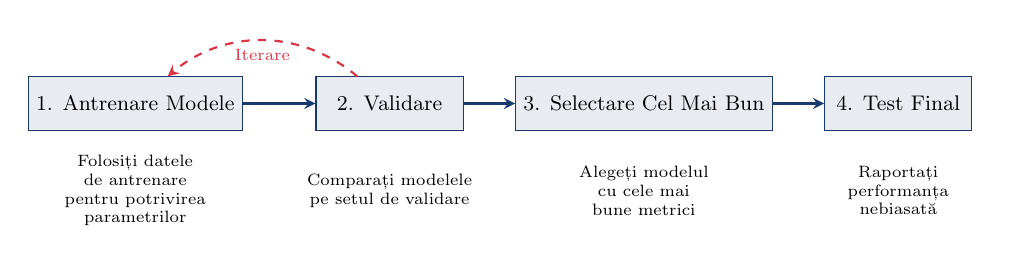
\begin{tikzpicture}[node distance=1.8cm, scale=0.85, transform shape]
        \tikzstyle{process} = [rectangle, minimum width=2.2cm, minimum height=0.8cm, text centered, draw=MainBlue, fill=MainBlue!10, font=\small]
        \tikzstyle{arrow} = [->, >=stealth, thick, MainBlue]

        % Noduri
        \node (train) [process] {1. Antrenare Modele};
        \node (validate) [process, right of=train, xshift=2cm] {2. Validare};
        \node (select) [process, right of=validate, xshift=2cm] {3. Selectare Cel Mai Bun};
        \node (test) [process, right of=select, xshift=2cm] {4. Test Final};

        % Săgeți
        \draw [arrow] (train) -- (validate);
        \draw [arrow] (validate) -- (select);
        \draw [arrow] (select) -- (test);

        % Buclă de feedback
        \draw [arrow, dashed, Crimson] (validate) to[bend right=40] node[below, font=\scriptsize] {Iterare} (train);

        % Etichete dedesubt
        \node [below of=train, yshift=0.5cm, font=\scriptsize, text width=2.5cm, align=center] {Folosiți datele de antrenare\\pentru potrivirea parametrilor};
        \node [below of=validate, yshift=0.5cm, font=\scriptsize, text width=2.5cm, align=center] {Comparați modelele\\pe setul de validare};
        \node [below of=select, yshift=0.5cm, font=\scriptsize, text width=2.5cm, align=center] {Alegeți modelul\\cu cele mai bune metrici};
        \node [below of=test, yshift=0.5cm, font=\scriptsize, text width=2.5cm, align=center] {Raportați performanța\\nebiasată};
    \end{tikzpicture}
    \end{center}

    \vspace{0.15cm}

    \begin{alertblock}{Regulă Critică}
        \textbf{Niciodată} nu folosiți setul de test pentru selecția modelului! Aceasta cauzează \textit{scurgere de date} și estimări excesiv de optimiste ale performanței.
    \end{alertblock}
\end{frame}

\begin{frame}{Date Reale: Compararea Prognozelor}
    \begin{center}
        \includegraphics[width=0.78\textwidth]{real_data_forecast_comparison.pdf}
    \end{center}
    \vspace{-0.2cm}
    \small Date pasageri aerieni: Holt-Winters Multiplicativ performează cel mai bine pentru date sezoniere.
\end{frame}

\begin{frame}{Performanța Prognozei pe Diferite Seturi de Date}
    \begin{center}
        \includegraphics[width=0.78\textwidth]{multiple_series_comparison.pdf}
    \end{center}
    \vspace{-0.2cm}
    \small Serii diferite necesită modele diferite. Datele sezoniere au nevoie de metode sezoniere.
\end{frame}

%=============================================================================
% SECȚIUNEA 5: MODELAREA SEZONALITĂȚII
%=============================================================================
\section{Modelarea Sezonalității}

\begin{frame}{Modelarea Sezonalității: Două Abordări}
    \begin{columns}[T]
        \begin{column}{0.48\textwidth}
            \textbf{1. Variabile Dummy:}

            \vspace{0.1cm}
            $X_t = \mu + \sum_{j=1}^{s-1}\gamma_j D_{jt} + \varepsilon_t$

            \vspace{0.2cm}
            \begin{itemize}
                \item $D_{jt} = 1$ dacă $t$ în sezonul $j$
                \item $s-1$ parametri
                \item Orice tipar sezonier
            \end{itemize}
        \end{column}
        \begin{column}{0.48\textwidth}
            \textbf{2. Termeni Fourier:}

            \vspace{0.1cm}
            $X_t = \mu + \sum_{k=1}^{K}[\alpha_k\sin(\cdot) + \beta_k\cos(\cdot)]$

            \vspace{0.2cm}
            \begin{itemize}
                \item Funcții sinusoidale
                \item $2K$ parametri
                \item Tipare netede
            \end{itemize}
        \end{column}
    \end{columns}

    \vspace{0.15cm}

    \begin{alertblock}{Compromis}
        Dummy: orice tipar, mai mulți parametri. Fourier: neted, mai puțini parametri.
    \end{alertblock}
\end{frame}

\begin{frame}{Variabile Dummy vs Termeni Fourier}
    \begin{center}
        \includegraphics[width=0.78\textwidth]{seasonality_fourier_dummies.pdf}
    \end{center}
\end{frame}

\begin{frame}{Alegerea între Dummy și Fourier}
    \begin{center}
    \small
    \begin{tabular}{lcc}
        \toprule
        \textbf{Criteriu} & \textbf{Dummy} & \textbf{Fourier} \\
        \midrule
        Parametri (lunar) & 11 & $2K$ (adesea 4--6) \\
        Tipar sezonier & Orice formă & Neted/sinusoidal \\
        Interpretare & Directă (efecte lunare) & Componente de frecvență \\
        Sezoane de înaltă frecvență & Mulți parametri & Eficient \\
        Sezonalitate multiplă & Complex & Ușor (adăugare termeni) \\
        \bottomrule
    \end{tabular}
    \end{center}

    \vspace{0.15cm}

    \textbf{Ghiduri:}
    \begin{itemize}
        \item Folosiți \textbf{dummy} când tiparul sezonier este neregulat sau aveți nevoie de coeficienți interpretabili
        \item Folosiți \textbf{Fourier} pentru tipare netede, sezonalitate de înaltă frecvență (zilnică, orară) sau perioade sezoniere multiple
        \item \textbf{Termenii Fourier} sunt folosiți în modelele TBATS și Facebook Prophet
    \end{itemize}
\end{frame}

%=============================================================================
% SECȚIUNEA 6: GESTIONAREA TRENDULUI ȘI SEZONALITĂȚII
%=============================================================================
\section{Gestionarea Trendului și Sezonalității}

\begin{frame}{De Ce Eliminăm Trendul și Sezonalitatea?}
    \textbf{Înainte de modelare}, adesea trebuie să facem seria staționară:

    \vspace{0.15cm}

    \begin{columns}[T]
        \begin{column}{0.48\textwidth}
            \textbf{Motive pentru detrendare:}
            \begin{itemize}
                \item Cerința de staționaritate
                \item Focus pe fluctuații
                \item Evitarea regresiei false
                \item Permiterea inferenței valide
            \end{itemize}
        \end{column}
        \begin{column}{0.48\textwidth}
            \textbf{Motive pentru desezonalizare:}
            \begin{itemize}
                \item Dezvăluirea trendului subiacent
                \item Comparare între sezoane
                \item Simplificarea modelării
                \item Focus pe componenta neregulată
            \end{itemize}
        \end{column}
    \end{columns}

    \vspace{0.2cm}

    \begin{alertblock}{Important}
        După modelarea seriei detrendate/desezonalizate, trebuie să \textbf{inversăm transformarea} pentru prognoză.
    \end{alertblock}
\end{frame}

\begin{frame}{Metode de Eliminare a Trendului}
    \textbf{Șase abordări comune de detrendare:}

    \vspace{0.2cm}

    \begin{enumerate}
        \item \textbf{Diferențiere}: $\Delta X_t = X_t - X_{t-1}$
        \item \textbf{Regresie liniară}: Potrivire $\hat{T}_t = \hat{\beta}_0 + \hat{\beta}_1 t$
        \item \textbf{Polinomială}: Potrivire polinom de ordin superior
        \item \textbf{Filtru HP}: Echilibru între potrivire și netezime
        \item \textbf{Media mobilă}: $\hat{T}_t = MA_q(X_t)$
        \item \textbf{LOESS}: Regresie polinomială locală
    \end{enumerate}

    \vspace{0.15cm}

    \textbf{Alegerea depinde de:}
    \begin{itemize}
        \item Natura trendului (determinist vs stocastic)
        \item Scopul (prognoză vs analiză)
    \end{itemize}
\end{frame}

\begin{frame}{Metode de Detrendare: Comparație}
    \begin{center}
        \includegraphics[width=0.78\textwidth]{detrending_methods.pdf}
    \end{center}
\end{frame}

\begin{frame}{Estimarea Trendului: Abordări Multiple}
    \begin{center}
        \includegraphics[width=0.78\textwidth]{trend_estimation_comparison.pdf}
    \end{center}
    \vspace{-0.2cm}
    \small Metodele diferite captează trendul la niveluri variate de netezime.
\end{frame}

\begin{frame}{Metode de Eliminare a Sezonalității}
    \textbf{Patru abordări pentru eliminarea sezonalității:}

    \vspace{0.15cm}

    \begin{enumerate}
        \item \textbf{Diferențiere sezonieră}: $\Delta_s X_t = X_t - X_{t-s}$

        \vspace{0.2cm}

        \item \textbf{Împărțire} (multiplicativ): $X_t^{adj} = X_t / \hat{S}_t$

        \vspace{0.2cm}

        \item \textbf{Scădere} (aditiv): $X_t^{adj} = X_t - \hat{S}_t$

        \vspace{0.2cm}

        \item \textbf{X-13ARIMA-SEATS}: Metodă statistică guvernamentală
    \end{enumerate}

    \vspace{0.15cm}

    \textbf{Perioada sezonieră} $s$: Lunar $\Rightarrow s=12$; Trimestrial $\Rightarrow s=4$
\end{frame}

\begin{frame}{Ajustare Sezonieră: Vizualizare}
    \begin{center}
        \includegraphics[width=0.78\textwidth]{seasonal_adjustment.pdf}
    \end{center}
\end{frame}

\begin{frame}{Trend Determinist vs Stocastic}
    \begin{columns}[T]
        \begin{column}{0.48\textwidth}
            \textbf{Trend Determinist:}
            \[
                X_t = \beta_0 + \beta_1 t + \varepsilon_t
            \]
            \begin{itemize}
                \item Trendul este o funcție de timp
                \item Detrendare prin regresie
                \item $\varepsilon_t$ este staționar
            \end{itemize}
        \end{column}
        \begin{column}{0.48\textwidth}
            \textbf{Trend Stocastic:}
            \[
                X_t = X_{t-1} + \varepsilon_t
            \]
            \begin{itemize}
                \item Componentă de mers aleatoriu
                \item Detrendare prin diferențiere
                \item $\Delta X_t$ este staționar
            \end{itemize}
        \end{column}
    \end{columns}

    \vspace{0.15cm}

    \begin{alertblock}{Metoda Greșită = Probleme}
        \begin{itemize}
            \item Diferențierea trendului determinist $\Rightarrow$ supra-diferențiere
            \item Regresie pe trend stocastic $\Rightarrow$ regresie falsă
        \end{itemize}
    \end{alertblock}
\end{frame}

\begin{frame}{Exemplu: Trend Determinist}
    \begin{center}
        \includegraphics[width=0.78\textwidth]{deterministic_trend_example.pdf}
    \end{center}
    \vspace{-0.1cm}
    \small \textbf{Cheie:} Folosiți \textcolor{Crimson}{regresia} pentru a elimina trendul $\rightarrow$ reziduurile sunt staționare (ACF scade rapid).
\end{frame}

\begin{frame}{Exemplu: Trend Stocastic (Mers Aleatoriu)}
    \begin{center}
        \includegraphics[width=0.78\textwidth]{stochastic_trend_example.pdf}
    \end{center}
    \vspace{-0.1cm}
    \small \textbf{Cheie:} Folosiți \textcolor{Crimson}{diferențierea} pentru a elimina trendul $\rightarrow$ diferențele sunt staționare (zgomot alb).
\end{frame}

\begin{frame}{Comparație Alăturată}
    \begin{center}
        \includegraphics[width=0.72\textwidth]{trend_comparison_sidebyside.pdf}
    \end{center}
    \vspace{-0.2cm}
    \small \textbf{Rețineți:} Determinist $\rightarrow$ regresie. Stocastic $\rightarrow$ diferențiere.
\end{frame}

%=============================================================================
% SECȚIUNEA 7: PROCESE STOCASTICE
%=============================================================================
\section{Procese Stocastice}

\begin{frame}{Proces Stocastic: Definiție}
    \begin{defn}[Proces Stocastic]
        Un \textbf{proces stocastic} este o colecție de variabile aleatoare indexate după timp:
        \[
            \{X_t(\omega) : t \in \mathcal{T}, \omega \in \Omega\}
        \]
        unde $\Omega$ este spațiul de selecție al rezultatelor posibile.
    \end{defn}

    \vspace{0.15cm}

    \textbf{Două perspective:}
    \begin{itemize}
        \item \textbf{$\omega$ fix}: O \textit{realizare} sau \textit{traiectorie de selecție} $\{X_t(\omega)\}_{t \in \mathcal{T}}$
        \item \textbf{$t$ fix}: O \textit{variabilă aleatoare} $X_t$ cu distribuția $F_t(x)$
    \end{itemize}

    \vspace{0.15cm}

    \textbf{Observație cheie:} O serie de timp pe care o observăm este \textbf{o realizare} a procesului stocastic subiacent. Folosim această singură realizare pentru a deduce proprietățile procesului.
\end{frame}

\begin{frame}{Proces Stocastic: Ilustrație Vizuală}
    \begin{center}
        \includegraphics[width=0.9\textwidth]{charts/ch1_def_stochastic.pdf}
    \end{center}
    \vspace{-0.2cm}
    \small Fiecare linie este o realizare diferită din același proces stocastic subiacent. Observăm doar o realizare dar vrem să înțelegem procesul.
\end{frame}

\begin{frame}{Momentele unui Proces Stocastic}
    \textbf{Primele două momente caracterizează proprietățile slabe:}

    \vspace{0.2cm}

    \textbf{Funcția de Medie:} \quad $\mu_t = \E[X_t]$

    \vspace{0.2cm}

    \textbf{Funcția de Autocovarianță (ACVF):}
    \[
        \gamma(t, s) = \Cov(X_t, X_s) = \E[(X_t - \mu_t)(X_s - \mu_s)]
    \]

    \vspace{0.2cm}

    \textbf{Funcția de Autocorelație (ACF):}
    \[
        \rho(t, s) = \frac{\gamma(t, s)}{\sqrt{\Var(X_t) \cdot \Var(X_s)}}
    \]

    \vspace{0.2cm}

    \textbf{Proprietăți:} $\rho(t, s) \in [-1, 1]$ și $\rho(t, t) = 1$
\end{frame}

%=============================================================================
% SECȚIUNEA 4: STAȚIONARITATEA
%=============================================================================
\section{Staționaritatea}

\begin{frame}{De Ce Contează Staționaritatea}
    \textbf{Staționaritatea} este o ipoteză fundamentală pentru analiza seriilor de timp:

    \vspace{0.15cm}

    \begin{columns}[T]
        \begin{column}{0.48\textwidth}
            \textbf{\textcolor{Crimson}{Fără Staționaritate:}}
            \begin{itemize}
                \item Media, varianța se schimbă în timp
                \item Trecutul poate să nu prezică viitorul
                \item Metodele standard eșuează
                \item Corelații false
            \end{itemize}
        \end{column}
        \begin{column}{0.48\textwidth}
            \textbf{\textcolor{Forest}{Cu Staționaritate:}}
            \begin{itemize}
                \item Proprietăți statistice constante
                \item Putem estima din o singură realizare
                \item Inferență validă posibilă
                \item Modelele sunt semnificative
            \end{itemize}
        \end{column}
    \end{columns}

    \vspace{0.2cm}

    \begin{alertblock}{Principiu Cheie}
        Majoritatea modelelor de serii de timp (ARMA, ARIMA, etc.) necesită staționaritate. Seriile nestaționare trebuie transformate (de ex., diferențiere) înainte de modelare.
    \end{alertblock}
\end{frame}

\begin{frame}{Staționar vs Nestaționar: Comparație Vizuală}
    \vspace{-0.3cm}
    \begin{center}
        \includegraphics[width=0.82\textwidth, height=0.58\textheight, keepaspectratio]{charts/ch1_stationarity.pdf}
    \end{center}
    \vspace{-0.2cm}
    {\footnotesize
    \begin{itemize}
        \item \textbf{Staționar}: Medie și varianță constante -- fluctuează în jurul unui nivel fix
        \item \textbf{Nestaționar}: Media și/sau varianța se schimbă în timp
        \item Inspecția vizuală este primul pas; testele formale (ADF, KPSS) confirmă
    \end{itemize}
    }
\end{frame}

\begin{frame}{Staționaritate Strictă}
    \begin{defn}[Staționaritate Strictă (Puternică)]
        Un proces $\{X_t\}$ este \textbf{strict staționar} dacă pentru toți $k$, toți $t_1, \ldots, t_k$ și toți $h$:
        \[
            (X_{t_1}, X_{t_2}, \ldots, X_{t_k}) \stackrel{d}{=} (X_{t_1+h}, X_{t_2+h}, \ldots, X_{t_k+h})
        \]
    \end{defn}

    \vspace{0.15cm}

    \textbf{Interpretare:} Distribuția comună a oricărei colecții de observații este \textbf{invariantă la deplasări temporale}.

    \vspace{0.15cm}

    \textbf{Implicații:}
    \begin{itemize}
        \item Toate distribuțiile marginale $F_{X_t}(x)$ sunt identice
        \item $\E[X_t] = \mu$ (medie constantă)
        \item $\Var(X_t) = \sigma^2$ (varianță constantă)
        \item Distribuțiile comune depind doar de \textit{diferențele} temporale
    \end{itemize}

    \vspace{0.2cm}

    \textbf{Notă:} Staționaritatea strictă este o condiție puternică, adesea impractică de verificat.
\end{frame}

\begin{frame}{Staționaritate Strictă: Ilustrație Vizuală}
    \begin{center}
        \includegraphics[width=0.95\textwidth]{charts/ch1_def_strict_stationarity.pdf}
    \end{center}
    \vspace{-0.2cm}
    \small Staționar: oricare două ferestre au aceeași distribuție comună. Nestaționar: distribuția se schimbă în timp.
\end{frame}

\begin{frame}{Staționaritate Slabă (de Covarianță)}
    \begin{defn}[Staționaritate Slabă]
        Un proces $\{X_t\}$ este \textbf{slab staționar} (sau staționar de covarianță) dacă:
        \begin{enumerate}
            \item $\E[X_t] = \mu$ \quad (medie constantă)
            \item $\Var(X_t) = \sigma^2 < \infty$ \quad (varianță constantă, finită)
            \item $\Cov(X_t, X_{t+h}) = \gamma(h)$ \quad (covarianța depinde doar de lag-ul $h$)
        \end{enumerate}
    \end{defn}

    \vspace{0.15cm}

    \textbf{Proprietate cheie:} Autocovarianța este o funcție doar de lag:
    \[
        \gamma(h) = \Cov(X_t, X_{t+h}) = \E[(X_t - \mu)(X_{t+h} - \mu)]
    \]

    \vspace{0.2cm}

    \textbf{Funcția de autocorelație:}
    \[
        \rho(h) = \frac{\gamma(h)}{\gamma(0)} = \frac{\Cov(X_t, X_{t+h})}{\Var(X_t)}
    \]

    Notă: $\rho(0) = 1$ și $\rho(h) = \rho(-h)$ (simetrie)
\end{frame}

\begin{frame}{Staționaritate Slabă: Ilustrație Vizuală}
    \begin{center}
        \includegraphics[width=0.95\textwidth]{charts/ch1_def_weak_stationarity.pdf}
    \end{center}
    \vspace{-0.2cm}
    \small Stânga: medie și varianță constante. Dreapta: autocovarianța depinde doar de lag-ul $h$, nu de timpul $t$.
\end{frame}

\begin{frame}{Proprietățile Funcției de Autocovarianță}
    Pentru un proces slab staționar, ACVF $\gamma(h)$ satisface:

    \vspace{0.15cm}

    \begin{enumerate}
        \item \textbf{Simetrie:} $\gamma(h) = \gamma(-h)$

        \vspace{0.2cm}

        \item \textbf{Maxim la zero:} $|\gamma(h)| \leq \gamma(0)$

        \vspace{0.2cm}

        \item \textbf{Definit nenegativ}
    \end{enumerate}

    \vspace{0.15cm}

    \textbf{Implicație:} Nu orice funcție poate fi o funcție de autocovarianță.
\end{frame}

%=============================================================================
% SECȚIUNEA 5: ZGOMOT ALB ȘI MERS ALEATORIU
%=============================================================================
\section{Zgomot Alb și Mers Aleatoriu}

\begin{frame}{Procesul de Zgomot Alb}
    \begin{defn}[Zgomot Alb]
        Un proces $\{\varepsilon_t\}$ este \textbf{zgomot alb}, notat $\varepsilon_t \sim WN(0, \sigma^2)$, dacă:
        \begin{enumerate}
            \item $\E[\varepsilon_t] = 0$ pentru toți $t$
            \item $\Var(\varepsilon_t) = \sigma^2$ pentru toți $t$
            \item $\Cov(\varepsilon_t, \varepsilon_s) = 0$ pentru $t \neq s$
        \end{enumerate}
    \end{defn}

    \vspace{0.2cm}

    \textbf{ACF al Zgomotului Alb:}
    \[
        \rho(h) = \begin{cases}
            1 & \text{dacă } h = 0 \\
            0 & \text{dacă } h \neq 0
        \end{cases}
    \]

    \vspace{0.2cm}

    \textbf{Tipuri:}
    \begin{itemize}
        \item \textbf{Zgomot alb slab}: Necorelat (condițiile de mai sus)
        \item \textbf{Zgomot alb puternic}: Independent și identic distribuit (i.i.d.)
        \item \textbf{Zgomot alb Gaussian}: $\varepsilon_t \stackrel{iid}{\sim} N(0, \sigma^2)$
    \end{itemize}
\end{frame}

\begin{frame}{Zgomot Alb vs Mers Aleatoriu: Comparație}
    \vspace{-0.3cm}
    \begin{center}
        \includegraphics[width=0.82\textwidth, height=0.58\textheight, keepaspectratio]{charts/ch1_wn_rw.pdf}
    \end{center}
    \vspace{-0.2cm}
    {\footnotesize
    \begin{itemize}
        \item \textbf{Zgomot alb}: Fluctuează în jurul lui zero -- staționar, varianță constantă
        \item \textbf{Mers aleatoriu}: Suma cumulativă a zgomotului alb -- rătăcește, nestaționar
        \item Mersul aleatoriu este cel mai simplu proces nestaționar (rădăcină unitate)
    \end{itemize}
    }
\end{frame}

\begin{frame}{Zgomot Alb: Ilustrație Vizuală}
    \begin{center}
        \includegraphics[width=0.95\textwidth]{charts/ch1_def_white_noise.pdf}
    \end{center}
    \vspace{-0.2cm}
    \small Stânga: zgomotul alb fluctuează în jurul lui zero cu varianță constantă. Dreapta: ACF arată nicio autocorelație (toate zero după lag 0).
\end{frame}

\begin{frame}{Procesul de Mers Aleatoriu}
    \textbf{Definiție:} $X_t = X_{t-1} + \varepsilon_t$ unde $\varepsilon_t \sim WN(0, \sigma^2)$, $X_0 = 0$

    \vspace{0.2cm}

    \textbf{Forma explicită:} $X_t = \sum_{i=1}^{t} \varepsilon_i$

    \vspace{0.15cm}

    \textbf{Proprietăți:}
    \begin{itemize}
        \item $\E[X_t] = 0$ (medie constantă)
        \item $\Var(X_t) = t\sigma^2$ (varianța crește în timp!)
        \item $\Cov(X_t, X_s) = \min(t, s) \cdot \sigma^2$
    \end{itemize}

    \vspace{0.15cm}

    \begin{alertblock}{Nestaționar!}
        Mersul aleatoriu \textbf{nu este staționar} deoarece varianța depinde de $t$.
    \end{alertblock}
\end{frame}

\begin{frame}{Mers Aleatoriu: Vizualizare}
    \begin{center}
        \includegraphics[width=0.78\textwidth]{random_walk.pdf}
    \end{center}
    \vspace{-0.2cm}
    \small \textbf{Stânga:} Traiectorii multiple divergă în timp. \textbf{Dreapta:} Varianța crește liniar: $\Var(X_t) = t\sigma^2$.
\end{frame}

\begin{frame}{Staționar vs Nestaționar: Comparație}
    \begin{center}
        \includegraphics[width=0.78\textwidth]{rw_vs_stationary.pdf}
    \end{center}
    \vspace{-0.2cm}
    \small\textbf{Diagnostic cheie:} ACF al procesului staționar scade rapid; ACF al mersului aleatoriu scade foarte lent.
\end{frame}

%=============================================================================
% SECȚIUNEA 6: ACF ȘI PACF
%=============================================================================
\section{Funcții de Autocorelație}

\begin{frame}{Funcția de Autocorelație din Eșantion}
    \textbf{ACF din eșantion la lag-ul $h$:}
    \[
        \hat{\rho}(h) = \frac{\sum_{t=1}^{T-h}(x_t - \bar{x})(x_{t+h} - \bar{x})}{\sum_{t=1}^{T}(x_t - \bar{x})^2}
    \]

    \vspace{0.15cm}

    \textbf{Proprietăți:}
    \begin{itemize}
        \item $\hat{\rho}(0) = 1$ întotdeauna
        \item $|\hat{\rho}(h)| \leq 1$
    \end{itemize}

    \vspace{0.15cm}

    \textbf{Test de semnificație:} Sub zgomot alb, $\hat{\rho}(h) \approx N(0, 1/T)$

    \vspace{0.2cm}

    \textbf{Limite 95\%:} $\pm 1.96/\sqrt{T}$
\end{frame}

\begin{frame}{Tipare ACF pentru Diferite Procese}
    \vspace{-0.3cm}
    \begin{center}
        \includegraphics[width=0.82\textwidth, height=0.58\textheight, keepaspectratio]{charts/ch1_acf_examples.pdf}
    \end{center}
    \vspace{-0.2cm}
    {\footnotesize
    \begin{itemize}
        \item \textbf{Zgomot alb}: ACF scade la zero imediat (nicio dependență)
        \item \textbf{AR(1)}: ACF scade exponențial -- indică structură autoregresivă
        \item \textbf{Sezonier}: ACF arată vârfuri la lag-uri sezoniere (de ex., 12, 24 pentru lunar)
        \item \textbf{Mers aleatoriu}: ACF scade foarte lent -- semn de nestaționaritate
    \end{itemize}
    }
\end{frame}

\begin{frame}{Funcția de Autocorelație Parțială (PACF)}
    \textbf{PACF} $\phi_{hh}$: Corelația dintre $X_t$ și $X_{t+h}$ după eliminarea efectului liniar al $X_{t+1}, \ldots, X_{t+h-1}$.

    \vspace{0.15cm}

    \textbf{Interpretare:}
    \begin{itemize}
        \item $\phi_{11} = \rho(1)$ (același ca ACF la lag 1)
        \item $\phi_{22} = $ corelația lui $X_t, X_{t+2}$ controlând pentru $X_{t+1}$
        \item Măsoară dependența \textit{directă} la lag-ul $h$
    \end{itemize}

    \vspace{0.15cm}

    \textbf{Aplicație cheie:} Identificarea ordinului AR
    \begin{itemize}
        \item Pentru AR($p$): PACF \textbf{se întrerupe} după lag-ul $p$
        \item Pentru MA($q$): ACF \textbf{se întrerupe} după lag-ul $q$
    \end{itemize}
\end{frame}

\begin{frame}{Tipare ACF și PACF}
    \begin{center}
        \includegraphics[width=0.72\textwidth]{acf_pacf_examples.pdf}
    \end{center}
\end{frame}

\begin{frame}{ACF Teoretic pentru AR(1)}
    \begin{center}
        \includegraphics[width=0.78\textwidth]{acf_theoretical.pdf}
    \end{center}
    \vspace{-0.2cm}
    \small Pentru AR(1): $X_t = \phi X_{t-1} + \varepsilon_t$, ACF teoretic este $\rho(h) = \phi^h$.
\end{frame}

%=============================================================================
% SECȚIUNEA 7: OPERATORUL LAG ȘI DIFERENȚIEREA
%=============================================================================
\section{Operatorul Lag și Diferențierea}

\begin{frame}{Operatorul Lag}
    \begin{defn}[Operatorul Lag]
        \textbf{Operatorul lag} (sau operatorul de întârziere) $L$ este definit prin:
        \[
            LX_t = X_{t-1}
        \]
    \end{defn}

    \vspace{0.2cm}

    \textbf{Proprietăți:}
    \begin{itemize}
        \item $L^k X_t = X_{t-k}$ (întârziere cu $k$ perioade)
        \item $L^0 = I$ (identitate)
        \item $(1 - \phi L)X_t = X_t - \phi X_{t-1}$
    \end{itemize}

    \vspace{0.2cm}

    \textbf{Exemple:}
    \begin{itemize}
        \item AR(1): $(1 - \phi L)X_t = \varepsilon_t$
        \item MA(1): $X_t = (1 + \theta L)\varepsilon_t$
        \item AR($p$): $(1 - \phi_1 L - \phi_2 L^2 - \cdots - \phi_p L^p)X_t = \varepsilon_t$
    \end{itemize}
\end{frame}

\begin{frame}{Operatorul Lag: Ilustrație Vizuală}
    \begin{center}
        \includegraphics[width=0.9\textwidth]{charts/ch1_def_lag_operator.pdf}
    \end{center}
    \vspace{-0.2cm}
    \small Operatorul lag $L$ deplasează fiecare observație înapoi cu o perioadă de timp: $LX_t = X_{t-1}$.
\end{frame}

\begin{frame}{Diferențierea}
    \textbf{Prima diferență:} $\Delta X_t = X_t - X_{t-1} = (1 - L)X_t$

    \vspace{0.15cm}

    \textbf{De ce diferențiem?}
    \begin{itemize}
        \item Elimină trendul și rădăcina unitate
        \item Mers aleatoriu: $\Delta X_t = \varepsilon_t$ (zgomot alb)
    \end{itemize}

    \vspace{0.15cm}

    \textbf{Proces integrat:} $X_t \sim I(d)$ dacă $\Delta^d X_t$ este staționar
    \begin{itemize}
        \item $I(0)$: Staționar (nu necesită diferențiere)
        \item $I(1)$: Necesită o diferențiere
        \item $I(2)$: Necesită două diferențieri
    \end{itemize}
\end{frame}

\begin{frame}{Efectul Diferențierii: S\&P 500}
    \begin{center}
        \includegraphics[width=0.72\textwidth]{differencing_effect.pdf}
    \end{center}
\end{frame}

%=============================================================================
% SECȚIUNEA 8: TESTAREA STAȚIONARITĂȚII
%=============================================================================
\section{Testarea Staționarității}

\begin{frame}{Testul Augmented Dickey-Fuller (ADF)}
    \textbf{Model:} $\Delta X_t = \alpha + \gamma X_{t-1} + \sum_{i=1}^{p} \delta_i \Delta X_{t-i} + \varepsilon_t$

    \vspace{0.15cm}

    \begin{columns}[T]
        \begin{column}{0.48\textwidth}
            \textbf{Ipoteze:}
            \begin{itemize}
                \item $H_0$: $\gamma = 0$ (rădăcină unitate)
                \item $H_1$: $\gamma < 0$ (staționar)
            \end{itemize}
        \end{column}
        \begin{column}{0.48\textwidth}
            \textbf{Statistica de test:}
            \[
                \tau = \frac{\hat{\gamma}}{SE(\hat{\gamma})}
            \]
        \end{column}
    \end{columns}

    \vspace{0.15cm}

    \textbf{Decizie:}
    \begin{itemize}
        \item $\tau <$ valoare critică $\Rightarrow$ Respingem $H_0$ $\Rightarrow$ \textcolor{Forest}{Staționar}
        \item $\tau \geq$ valoare critică $\Rightarrow$ \textcolor{Crimson}{Nestaționar}
    \end{itemize}

    \vspace{0.2cm}
    \small Valori critice: distribuția Dickey-Fuller (nu normală)
\end{frame}

\begin{frame}{Testul KPSS}
    \textbf{Model:} $X_t = \xi t + r_t + \varepsilon_t$ unde $r_t = r_{t-1} + u_t$

    \vspace{0.2cm}

    \begin{columns}[T]
        \begin{column}{0.48\textwidth}
            \textbf{Ipoteze (opuse față de ADF):}
            \begin{itemize}
                \item $H_0$: $\sigma_u^2 = 0$ (staționar)
                \item $H_1$: $\sigma_u^2 > 0$ (rădăcină unitate)
            \end{itemize}
        \end{column}
        \begin{column}{0.48\textwidth}
            \textbf{Statistica de test:}
            \[
                LM = \frac{\sum_{t=1}^{T} S_t^2}{T^2 \hat{\sigma}^2}
            \]
            {\small unde $S_t = \sum_{i=1}^{t} \hat{e}_i$}
        \end{column}
    \end{columns}

    \vspace{0.2cm}

    \textbf{Decizie:}
    \begin{itemize}
        \item $LM >$ valoare critică $\Rightarrow$ Respingem $H_0$ $\Rightarrow$ \textcolor{Crimson}{Nestaționar}
        \item $LM \leq$ valoare critică $\Rightarrow$ \textcolor{Forest}{Staționar}
    \end{itemize}

    \vspace{0.1cm}
    \small \textbf{Notă:} KPSS complementează ADF---folosiți ambele pentru concluzii robuste.
\end{frame}

\begin{frame}{Folosirea ADF și KPSS Împreună}
    \textbf{Testare confirmatorie} pentru concluzii robuste:

    \vspace{0.15cm}

    \begin{center}
    \begin{tabular}{lccl}
        \toprule
        \textbf{ADF} & \textbf{KPSS} & \textbf{Concluzie} \\
        \midrule
        Respingem $H_0$ & Nu respingem $H_0$ & \textcolor{Forest}{Staționar} \\
        Nu respingem $H_0$ & Respingem $H_0$ & \textcolor{Crimson}{Rădăcină Unitate} \\
        Respingem $H_0$ & Respingem $H_0$ & Neconcludent \\
        Nu respingem $H_0$ & Nu respingem $H_0$ & Neconcludent \\
        \bottomrule
    \end{tabular}
    \end{center}

    \vspace{0.15cm}

    \textbf{Flux de lucru recomandat:}
    \begin{enumerate}
        \item Rulați testul ADF (nulă = rădăcină unitate)
        \item Rulați testul KPSS (nulă = staționar)
        \item Dacă rezultatele coincid, procedați cu încredere
        \item Dacă neconcludent, considerați teste alternative (PP, DF-GLS)
    \end{enumerate}
\end{frame}

\begin{frame}{Testul ADF: Vizualizare cu S\&P 500}
    \begin{center}
        \includegraphics[width=0.78\textwidth]{adf_test_visualization.pdf}
    \end{center}
\end{frame}

%=============================================================================
% SECȚIUNEA 9: APLICAȚIE PE DATE REALE
%=============================================================================
\section{Aplicație pe Date Financiare}

\begin{frame}{Analiza S\&P 500: Prezentare Generală}
    \begin{center}
        \includegraphics[width=0.78\textwidth]{sp500_analysis.pdf}
    \end{center}
\end{frame}

\begin{frame}{Fapte Stilizate ale Randamentelor Financiare}
    \begin{center}
        \includegraphics[width=0.78\textwidth]{returns_distribution.pdf}
    \end{center}

    \vspace{0.1cm}
    \begin{columns}[T]
        \begin{column}{0.48\textwidth}
            \textbf{Proprietăți observate:}
            \begin{itemize}
                \item Asimetrie negativă (coadă stângă)
                \item Kurtoză excesivă ($\gg 3$)
                \item Cozi groase (heavy tails)
            \end{itemize}
        \end{column}
        \begin{column}{0.48\textwidth}
            \textbf{Implicații:}
            \begin{itemize}
                \item Distribuția normală inadecvată
                \item Evenimente extreme mai probabile
                \item Necesită distribuție Student-t sau similară
            \end{itemize}
        \end{column}
    \end{columns}
\end{frame}

\begin{frame}{Gruparea Volatilității}
    \begin{center}
        \includegraphics[width=0.78\textwidth]{volatility_clustering.pdf}
    \end{center}

    \vspace{0.1cm}
    \begin{alertblock}{Fapt Stilizat}
        Randamentele mari (pozitive sau negative) tind să fie urmate de randamente mari. Această \textbf{grupare a volatilității} motivează modelele ARCH/GARCH (capitolele viitoare).
    \end{alertblock}
\end{frame}

%=============================================================================
% SECȚIUNEA 10: REZUMAT
%=============================================================================
\section{Rezumat}

\begin{frame}{Concluzii Cheie}
    \small
    \begin{enumerate}
        \item \textbf{Serie de timp} = observații indexate după timp cu dependență temporală
        \vspace{0.05cm}
        \item \textbf{Descompunere}: Aditivă $X_t = T_t + S_t + \varepsilon_t$ sau Multiplicativă
        \vspace{0.05cm}
        \item \textbf{Netezire Exponențială}: SES (nivel), Holt (trend), Holt-Winters (sezonier)
        \vspace{0.05cm}
        \item \textbf{Evaluare Prognoză}: MAE, RMSE, MAPE; folosiți separări train/validare/test
        \vspace{0.05cm}
        \item \textbf{Modelarea Sezonalității}: Variabile dummy (orice tipar) sau termeni Fourier (neted)
        \vspace{0.05cm}
        \item \textbf{Gestionarea Trendului}: Diferențiere (stocastic) sau regresie (determinist)
        \vspace{0.05cm}
        \item \textbf{Staționaritate}: Media, varianța, autocovarianța constante în timp
        \vspace{0.05cm}
        \item \textbf{ACF/PACF}: Esențiale pentru identificarea structurii de dependență
        \vspace{0.05cm}
        \item \textbf{Teste rădăcină unitate}: ADF ($H_0$: rădăcină unitate) vs KPSS ($H_0$: staționar)
    \end{enumerate}
\end{frame}

\begin{frame}{Formule Importante I}
    \begin{block}{Descompunere}
        Aditivă: $X_t = T_t + S_t + \varepsilon_t$ \quad Multiplicativă: $X_t = T_t \times S_t \times \varepsilon_t$
    \end{block}

    \begin{block}{Netezire Exponențială Simplă (SES)}
        $\hat{X}_{t+1|t} = \alpha X_t + (1-\alpha)\hat{X}_{t|t-1}$ \quad unde $\alpha \in (0,1)$
    \end{block}

    \begin{block}{Trend Liniar Holt}
        $\ell_t = \alpha X_t + (1-\alpha)(\ell_{t-1} + b_{t-1})$ \quad $b_t = \beta^*(\ell_t - \ell_{t-1}) + (1-\beta^*)b_{t-1}$
    \end{block}

    \begin{block}{Holt-Winters Aditivă}
        $\ell_t = \alpha(X_t - S_{t-s}) + (1-\alpha)(\ell_{t-1} + b_{t-1})$ \quad $S_t = \gamma(X_t - \ell_t) + (1-\gamma)S_{t-s}$
    \end{block}
\end{frame}

\begin{frame}{Formule Importante II}
    \begin{block}{Media Mobilă (Estimare Trend)}
        $\hat{T}_t = \frac{1}{2q+1}\sum_{j=-q}^{q} X_{t+j}$
    \end{block}

    \begin{block}{Autocovarianță și Autocorelație}
        $\gamma(h) = \Cov(X_t, X_{t+h})$ \qquad $\rho(h) = \frac{\gamma(h)}{\gamma(0)}$
    \end{block}

    \begin{block}{Mers Aleatoriu}
        $X_t = X_{t-1} + \varepsilon_t$ \quad $\Rightarrow$ \quad $\Var(X_t) = t\sigma^2$ (nestaționar)
    \end{block}

    \begin{block}{Diferențiere}
        $\Delta X_t = (1-L)X_t = X_t - X_{t-1}$
    \end{block}
\end{frame}

\begin{frame}{Previzualizare Capitolul Următor}
    \textbf{Capitolul 2: Modele ARMA}

    \vspace{0.2cm}

    \begin{itemize}
        \item Modele Autoregresive (AR)
        \item Modele de Medie Mobilă (MA)
        \item Modele ARMA combinate
        \item Identificarea modelului folosind ACF/PACF
        \item Estimarea parametrilor
        \item Diagnosticarea modelului
        \item Prognoza
    \end{itemize}
\end{frame}

%=============================================================================
% SECȚIUNEA: QUIZ
%=============================================================================
\section{Quiz}

\begin{frame}{Întrebarea Quiz 1}
    \begin{alertblock}{Întrebare}
        O serie de timp $Y_t$ arată mișcare ascendentă de-a lungul anilor plus tipare repetitive în fiecare trimestru. Ce componente sunt prezente?
    \end{alertblock}

    \vspace{0.3cm}

    \begin{enumerate}[(A)]
        \item Doar trend
        \item Doar sezonalitate
        \item Trend și Sezonalitate
        \item Doar zgomot aleatoriu
    \end{enumerate}
\end{frame}

\begin{frame}{Întrebarea Quiz 1: Răspuns}
    \begin{exampleblock}{Răspuns Corect: (C) Trend și Sezonalitate}
        Mișcare ascendentă = Trend; Tipare trimestriale = Sezonalitate (s=4)
    \end{exampleblock}
    \vspace{0.2cm}
    \begin{center}
        \includegraphics[width=0.95\textwidth, height=0.55\textheight, keepaspectratio]{charts/ch1_quiz1_components.pdf}
    \end{center}
\end{frame}

\begin{frame}{Întrebarea Quiz 2}
    \begin{alertblock}{Întrebare}
        Care dintre următoarele este o caracteristică a unei serii de timp staționare?
    \end{alertblock}

    \vspace{0.3cm}

    \begin{enumerate}[(A)]
        \item Media se schimbă în timp
        \item Varianța crește în timp
        \item Medie și varianță constante în timp
        \item Conține o componentă de trend
    \end{enumerate}
\end{frame}

\begin{frame}{Întrebarea Quiz 2: Răspuns}
    \begin{exampleblock}{Răspuns Corect: (C) Medie și varianță constante în timp}
        Staționaritatea necesită: medie constantă, varianță constantă și autocovarianța depinde doar de lag.
    \end{exampleblock}
    \vspace{0.2cm}
    \begin{center}
        \includegraphics[width=0.95\textwidth, height=0.55\textheight, keepaspectratio]{charts/ch1_quiz2_stationarity.pdf}
    \end{center}
\end{frame}

\begin{frame}{Întrebarea Quiz 3}
    \begin{alertblock}{Întrebare}
        Pentru un proces de zgomot alb, cum arată ACF la lag-uri $k > 0$?
    \end{alertblock}

    \vspace{0.3cm}

    \begin{enumerate}[(A)]
        \item Descreștere exponențială
        \item Toate valorile semnificative și pozitive
        \item Toate valorile aproximativ zero (în interiorul benzilor de încredere)
        \item Alternare pozitiv și negativ
    \end{enumerate}
\end{frame}

\begin{frame}{Întrebarea Quiz 3: Răspuns}
    \begin{exampleblock}{Răspuns Corect: (C) Aproximativ zero în interiorul benzilor de încredere}
        Zgomotul alb nu are autocorelație: $\rho_k = 0$ pentru toți $k \neq 0$.
    \end{exampleblock}
    \vspace{0.2cm}
    \begin{center}
        \includegraphics[width=0.95\textwidth, height=0.55\textheight, keepaspectratio]{charts/ch1_quiz3_acf.pdf}
    \end{center}
\end{frame}

\begin{frame}{Întrebarea Quiz 4}
    \begin{alertblock}{Întrebare}
        Care este diferența cheie între zgomotul alb și mersul aleatoriu?
    \end{alertblock}

    \vspace{0.3cm}

    \begin{enumerate}[(A)]
        \item Zgomotul alb are trend, mersul aleatoriu nu
        \item Mersul aleatoriu este suma cumulativă a zgomotului alb
        \item Ambele sunt procese staționare
        \item Zgomotul alb are varianță mai mare
    \end{enumerate}
\end{frame}

\begin{frame}{Întrebarea Quiz 4: Răspuns}
    \begin{exampleblock}{Răspuns Corect: (B) Mers aleatoriu = suma cumulativă a zgomotului alb}
        $Y_t = Y_{t-1} + \varepsilon_t = \sum_{i=1}^t \varepsilon_i$ unde $\varepsilon_t$ este zgomot alb.
    \end{exampleblock}
    \vspace{0.2cm}
    \begin{center}
        \includegraphics[width=0.95\textwidth, height=0.55\textheight, keepaspectratio]{charts/ch1_quiz4_wn_rw.pdf}
    \end{center}
\end{frame}

\begin{frame}{Întrebarea Quiz 5}
    \begin{alertblock}{Întrebare}
        Care metrică de eroare a prognozei este cea mai sensibilă la erori mari (valori aberante)?
    \end{alertblock}

    \vspace{0.3cm}

    \begin{enumerate}[(A)]
        \item MAE (Eroarea Medie Absolută)
        \item RMSE (Rădăcina Erorii Medii Pătratice)
        \item MAPE (Eroarea Medie Absolută Procentuală)
        \item Toate sunt la fel de sensibile
    \end{enumerate}
\end{frame}

\begin{frame}{Întrebarea Quiz 5: Răspuns}
    \begin{exampleblock}{Răspuns Corect: (B) RMSE}
        RMSE ridică la pătrat erorile, deci erorile mari au impact disproporționat: $\sqrt{\frac{1}{n}\sum e_t^2}$
    \end{exampleblock}
    \vspace{0.2cm}
    \begin{center}
        \includegraphics[width=0.95\textwidth, height=0.55\textheight, keepaspectratio]{charts/ch1_quiz5_forecast_errors.pdf}
    \end{center}
\end{frame}

\begin{frame}{Întrebarea Quiz 6}
    \begin{alertblock}{Întrebare}
        Când ar trebui să folosiți descompunerea multiplicativă în loc de cea aditivă?
    \end{alertblock}

    \vspace{0.3cm}

    \begin{enumerate}[(A)]
        \item Când seria nu are trend
        \item Când amplitudinea sezonieră este constantă
        \item Când amplitudinea sezonieră crește odată cu nivelul seriei
        \item Când seria este staționară
    \end{enumerate}
\end{frame}

\begin{frame}{Întrebarea Quiz 6: Răspuns}
    \begin{exampleblock}{Răspuns Corect: (C) Amplitudinea sezonieră crește odată cu nivelul}
        Multiplicativă: $Y_t = T_t \times S_t \times \varepsilon_t$ --- oscilațiile sezoniere proporționale cu trendul.
    \end{exampleblock}
    \vspace{0.2cm}
    \begin{center}
        \includegraphics[width=0.95\textwidth, height=0.55\textheight, keepaspectratio]{charts/ch1_quiz6_decomposition.pdf}
    \end{center}
\end{frame}

\begin{frame}{}
    \centering
    \Huge\textcolor{MainBlue}{Vă Mulțumesc!}

    \vspace{1cm}

    \Large Întrebări?

    \vspace{1cm}

    \normalsize
    Toate graficele generate folosind Python (yfinance, statsmodels, matplotlib)

    \vspace{0.15cm}

    Sursă date: Yahoo Finance (2019--2025)
\end{frame}

\end{document}
